%%%%%%%%%%%%%%%%%%%%%%%%%%%%%%%%%%%%%%%%%%%
\subsection{Архитектура.}
%%%%%%%%%%%%%%%%%%%%%%%%%%%%%%%%%%%%%%%%%%%
\begin{frame}%[allowframebreaks=0.9,t]

    В структуре программы почти любого компилятора можно выделить следующие части:

    \begin{figure}[H]
        \centering
        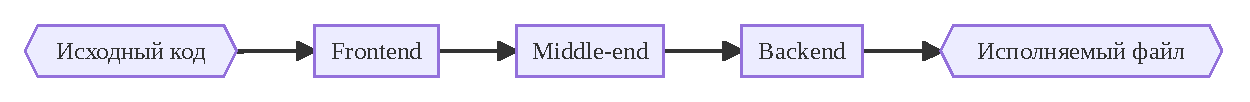
\includegraphics[width=\textwidth]{figures/arch}
        \caption{Архитектура большинства современных компиляторов}
        \label{fig:arch}
    \end{figure}

    Проект разрабатывается с использованием языка программирования Rust.
    Этот язык предлагает надежный концепт управления памятью, не имея при этом сборщика мусора.
    Кроме того, он соперничает по скорости с C и C++ и применяется в довольно широком спектре приложений.

\end{frame}

\begin{frame}
    Разбиение проекта на модули с указанием потока данных:
    \begin{figure}[H]
        \centering
        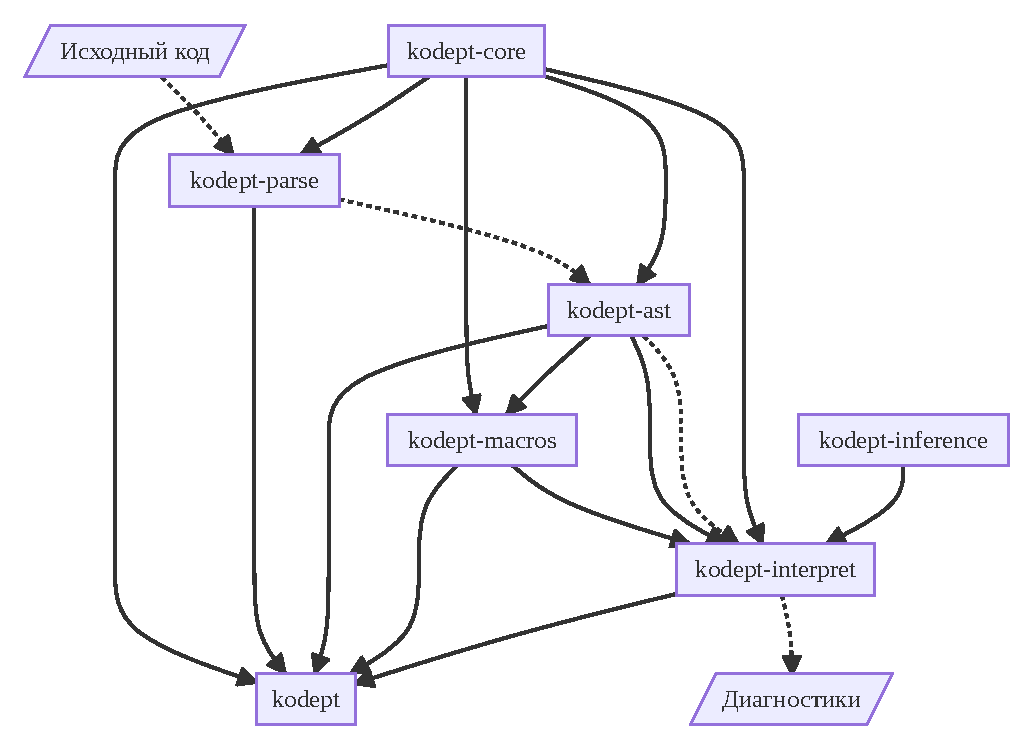
\includegraphics[height=0.7\textheight]{figures/modules}
        \caption{Иерархия модулей в проекте}
        \label{fig:modules}
    \end{figure}
\end{frame}
%%%%%%%%%%%%%%%%%%%%%%%%%%%%%%%%%%%%%%%%%%%
\subsection{Алгоритм W.}
%%%%%%%%%%%%%%%%%%%%%%%%%%%%%%%%%%%%%%%%%%%%%%%

\begin{frame}[fragile]
    Алгоритм W является одной из реализаций системы типов Хиндли-Милнера.

    \begin{columns}
        \begin{column}{0.6\textwidth}
            \begin{figure}
                \centering
                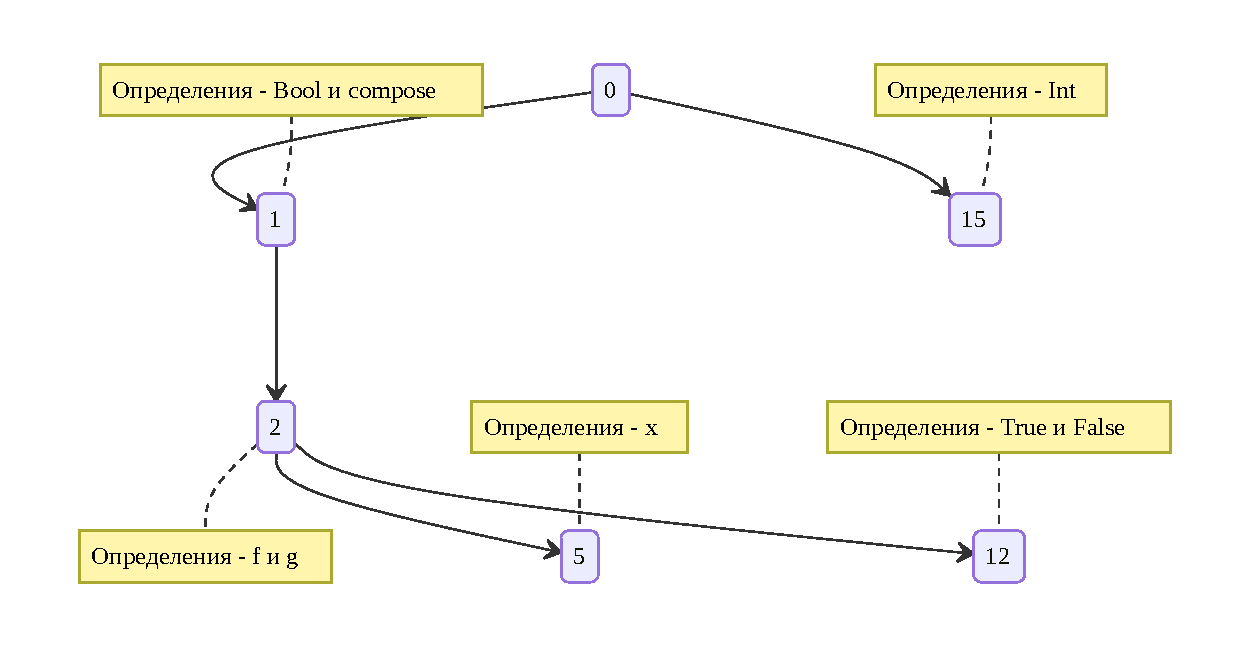
\includegraphics[width=\textwidth]{figures/scopes}
                \caption{Дерево областей видимости}
                \label{fig:scopes}
            \end{figure}
        \end{column}
        \begin{column}{0.4\textwidth}
            Разбиение на области видимости позволяет убедиться, что внутри области не используются неизвестные переменные или функции.

            \small{
            \begin{lstlisting}[label=lst:kodept, caption={Исходная программа на языке Kodept}]
module Testing {
    fun compose(f, g) => \x => f(g(x))
    enum struct Bool { True, False }
}
module Testing2 {
    struct Int
}
            \end{lstlisting}}
        \end{column}
    \end{columns}
\end{frame}
%%%%%%%%%%%%%%%%%%%%%%%%%%%%%%%%%%%%%%%%%%%%%%%
